\documentclass{beamer}
\newcommand{\myfont}{\rmfamily\normalsize\upshape\mdseries}
\newcommand{\degree}{^\circ}
\title{\sffamily Final Rivew -  Part I}
\subtitle{\textbf{Basic Graph Theory}\\Be sure to memorize the terminologies well...}
\institute[UM-SJTU JI]{University of Michigan-Shanghai Jiao Tong University Joint Institute}
\author{HamHam}
\usepackage{graphicx}
\usepackage{picinpar}
\usepackage{indentfirst}
\usepackage{chemformula}
\usepackage{geometry}
\usepackage{subfigure}
\usepackage{appendix}
\usepackage{amsfonts}
\usepackage{enumerate}
\usepackage{float}
\usepackage{geometry}
\usepackage{latexsym}
\usepackage{listings}
\usepackage{multicol,multirow,multido}
\usepackage{tabularx}
\usepackage{ulem}
\usepackage{tikz}
\usepackage{xcolor}
\usepackage{cite}
\usepackage{setspace}
\usepackage{hyperref}
\usepackage{textpos}
\usepackage{booktabs}
\usepackage{diagbox}
\usepackage{listings}
\usepackage{graphics}
\usepackage{upgreek}
\usepackage{JI_MathCourse_Notations}
\usepackage{mathrsfs}
\usepackage[final]{pdfpages}
%\usepackage{boondox-cal}
\usepackage{dutchcal}
\usepackage{colortbl}
%\usepackage{ctex} %插入中文
%\ctexset{today=old}

\newcommand{\mydef}[1]{\sffamily\blue{#1}\myfont\\} %for define
\newcommand{\mysol}{\yellow{Solution:}\\}
\usetheme[dove]{Boadilla}
\usecolortheme{dolphin}
\useoutertheme{miniframes}
\begin{document}
    \usebackgroundtemplate{\tikz\node[opacity=0.25]{
    
\includegraphics[width=\paperwidth,
    height=\paperheight]{hamster.jpg}
    };}
\begin{titlepage}
    \begin{center}
        VE203 - Discrete Mathmatics 
    \end{center}
\end{titlepage}
\myfont
\newcommand{\binomial}[2]{\begin{pmatrix} {#1}\\{#2}	\end{pmatrix}}
\newcommand{\green}[1]{\textcolor[rgb]{0.3,0.6,0}{#1}}
\definecolor{mygray}{gray}{.9}
\newcommand{\tg}[1]{\textbf{\green{{#1}}}}
\section{Terminology}

\begin{frame}{Terminology}
    \begin{block}{Graph Definition}
        \hh A \tg{graph} $G := \(V, E\)$ consists of set of \tg{vertices} $V\(G\)$ and 
    \tg{edges} $E\(G\)$, together with a relation indicating each edge 
    \tg{incident} with one or two vertices. Two vertices are called \tg{adjacent} if they are
    connected by at least one edge.
    \end{block}
    \vs{2em}
    \begin{block}{Simple Graph}
        An edge with just one end is called a \tg{loop}. Two distinct edges
    with the same ends are \tg{parallel}. A graph without loops or parallel
    edges is called \tg{simple}.
    \end{block}
\end{frame}
\begin{frame}
    \frametitle{Terminology}
    \hh There are two important relations and for graphs. Hmm, perhaps give some 
    examples?
    \begin{block}{Isomorphism}
    \hh An \tg{isomorphism} between simple graph $G$ and $H$ is a bijection
    $f : V\(G\) \to V\(H\)$ such that $u v \in E\(G\) \LRarrow f\(u\)f\(v\) \in E\(H\)$. In other
    words, f \textbf{preserves the structure} of $G$ and $H$. If such $f$ exists, we say
    $G$ is isomorphic to $H$, or $G \cong H$. 
    \par \hh Isomorphism is an \textbf{equivalence} relation between graphs.
    \end{block}
    \begin{block}{Subgrpah}
        \hh If $V\(H\) \subset V\(G\)$ and $E\(H\) \subset E\(G\)$ and $G$ and $H$ shares the same
        incidence relation, we say $H$ is a \tg{subgraph} of G, or $H \subset G$.
        \par \hh This forms a \textbf{partial order} between graphs.         
    \end{block}
\end{frame}
\begin{frame}
    \frametitle{Terminology}
    \begin{block}{Complement}
    \hh  The \tg{complement} $\overline{G}$ of a simple graph $G$ is the simple graph with
    vertex set $V\(G\)$ defined by $uv \in E\(\overline{G}\)$ iff 
    $uv  \not\in E\(G\)$. Note that given graph $G = \(V, E\)$, 
    we have $\overline{G} =\(V,\binom{v}{2} -  E\)$.
    \par \hh 
    A graph $G$ is said to be \tg{self-complementary} if $G \cong \overline{G}$.
    \end{block}
    \begin{block}{Null Graph}
        \hh The \tg{null graph} is the graph whose vertex set and edge set are
        empty, namely $G = \(\varnothing,\varnothing\)$.
    \end{block}
    \begin{block}{Clique}
    \hh  A \tg{clique} in a graph is a set of pairwise adjacent vertices.
    \end{block}
\end{frame}
\begin{frame}
    \frametitle{Exercise}
    1. Given a graph $G$ as follows:
    \begin{figure}
        \centering
        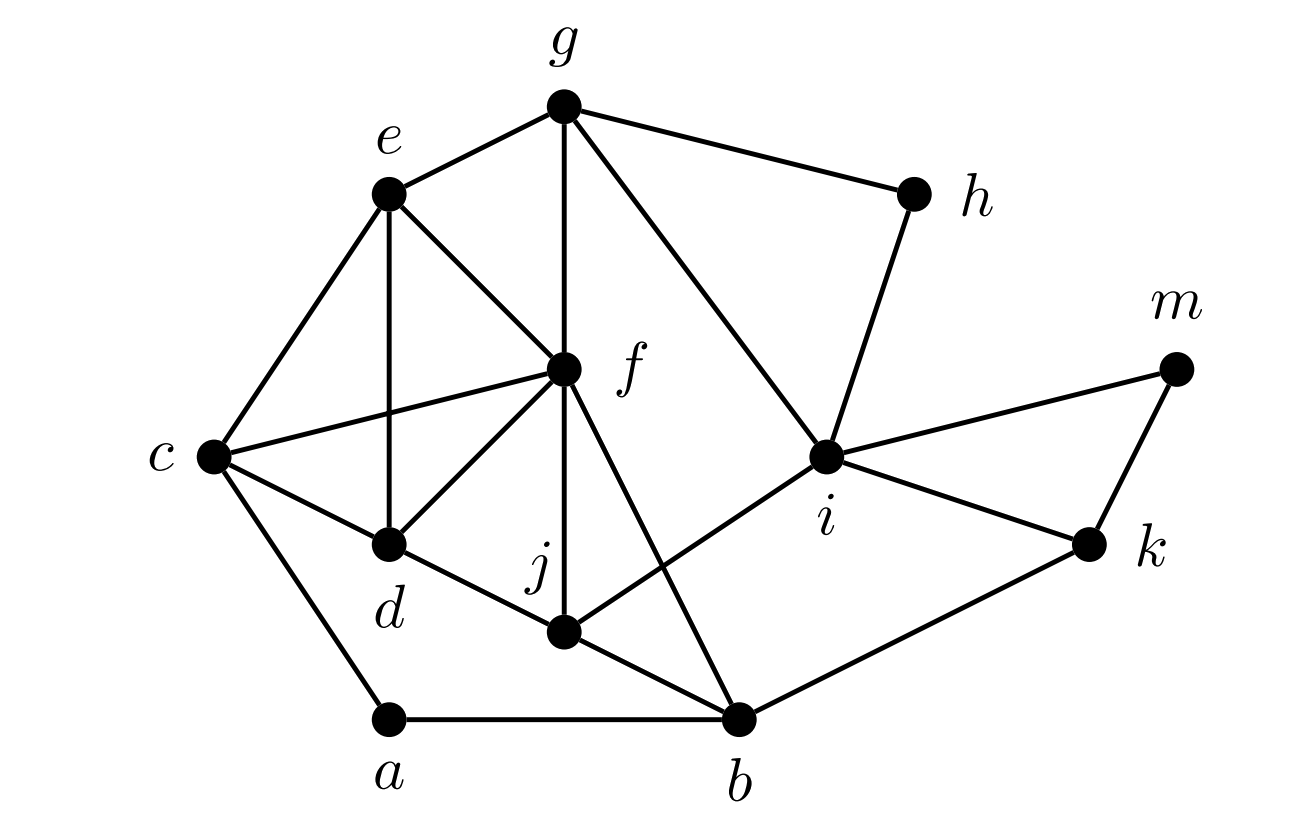
\includegraphics[scale=0.36]{graph2.png}
    \end{figure}
    See the questions in last semester's exam!
\end{frame}

\begin{frame}
    \frametitle{Standard Graph}
    \begin{block}{Complete Graph}
    \hh    A \tg{complete graph} with $n$ vertices $K_n := \(V, E\)$ satisfies
    $E =\binom{V}{2}$. If a subgraph of a graph is complete, its vertices are called a clique in this graph.
    \end{block}
    \begin{block}{Path}
    \hh A \tg{path} with $n$ vertices is 
    $P_n := \(\{v_i\}_{i=1}^n,\{v_i v_{i+1}\}_{i=1}^{n-1}\)$
    , where $i \neq j \Rightarrow v_i  \neq v_j$.
    \end{block}
    \begin{block}{Cycle}
    \hh    A \tg{cycle} with $n$ vertices is
    $C_n := \(\{v_i\}_{i=1}^n,\{v_i v_{i+1}\}_{i=1}^{n-1} \cup \{v_n v_1\}\)$, 
    where $i \neq  j \Rightarrow v_i \neq v_j$.
    \par 
    \hh Are $C_1$ and $C_2$ still simple graphs?
    \end{block}
\end{frame}
\begin{frame}
    \frametitle{The Handshaking Theorem}
    Undirected graph:
    $$2|E| = \sum_{v\in V}\deg(v)$$
    Directed graph:
    $$|E| = \sum_{v\in V} \deg^+ (v) = \sum_{v\in V} \deg^- (v)$$
    \green{Remark:}\\
    \begin{itemize}
        \item A vertex is said to be isolated if it has degree zero.
        \item A vertex is said to be pendant if it has degree one.
        \item $\deg^+(v)$: in-degree of a vertex v
        \item $\deg^-(v)$: out-degree of a vertex v
    \end{itemize}
\end{frame}
\begin{frame}
    \frametitle{Exercise}
    A little bit tricky exercise! But possible to appear in the exam!
    \par \vv
    2. Which of the following statements about graphs are correct?
    \begin{itemize}
        \item[(A)] $C_5$ is self-complementary.
        \item[(B)] $P_4$ is self-complementary
        \item[(C)] $K_{2,2}$ is induced in $C_4$.
        \item[(D)] $C_1$ is induced in $K_5$.
    \end{itemize}
    \vs{2em}
    \yellow{Answer:} 
    \textcolor[cmyk]{0.01,0.01,0.01,0.01}{A~B~C~} 
\end{frame}
\section{Connectivity}

\begin{frame}
    \frametitle{Walks and Connectivity}
    \mydef{Definition}
    \hh A \blue{walk} $W$ in $G$ is a sequence of vertices
    \green{$\{v_i\}^n_{i=0}$} and edges 
    \green{$\{e_i\}^n_{i=1}$} so that $e_i$
    is incident with $v_{i-1}$ and $v_i$. 
    \begin{itemize}
        \item $W$ is 
        called \textbf{closed} if $v_n=v_0$
        \item The \textbf{length} of $W$ is its number
        of edges $n$
        \item $G $ is connected if $\forall u,v \in V\(G\)$,
        there is a walk from $u$ to $v$
        \item A walk is generally \textbf{not} a graph, why?
    \end{itemize} 
\end{frame}
\begin{frame}
    \frametitle{Components}
    \mydef{Definition}
    \hh A component of a graph $G$ is a 
    \textbf{maximal connected subgraph} in
    $G$. In other words, it is not contained in any other connected
    subgraphs. 
    \\ \hh The number of components of $G$ is denoted as
    $\operatorname{comp}\(G\)$.
    \\
    \mydef{Theorem}
    \hh Every vertex is in a \textbf{unique} component.
    \begin{block}{Note}
        \hh If a graph $G$ isn't connected, it may be useful
        to consider its components.
    \end{block}
\end{frame}
\begin{frame}
    \frametitle{Cuts}
    \mydef{Definition(substraction)}
    \hh Given $G = \(V, E\)$, $S \subset E$, $X \subset V$, 
    then $G - S := \(V, E~\cut~S\)$ and
    $G - X := (V~\cut~ X, \{e \in E : e \text{ not incident with }x \in X\})$.
    \\ \vv
    \mydef{Definition}
    \begin{itemize}
        \item $e \in E$ is a \textbf{cut-edge } or \textbf{bridge} 
        if no cycle contains $e$
        \item $v \in V $ is a \textbf{cut-vertex} if 
         $\comp{G-v} > \comp{G}$
    \end{itemize}
    \green{What happens when we delete an edge or vertex?}
    \begin{itemize}
        \item If $e$ is a cut-edge, $\comp{G-e}=\comp{G}+1$
        \item If $e$ is not, $\comp{G-e}=\comp{G}$
        \item Further, $\comp{G-v} \leq \comp{G} + \deg\(v\) -1$
    \end{itemize}
    \green{Induced subgraph}
    \\ \hh \red{Please remember to delete both the vertexes and the edges!}
\end{frame}
\begin{frame}
    \frametitle{Exercise}
    3. A graph $G$ is called \tg{$k$-regular} if all 
    vertices of $G$ have the same degree $k$.
    \begin{itemize}
        \item[(i)] Show that a $k$-regular bipartite graph has no cut-edge for $k \geq 2$.
        \item[(ii)] Show that a $k$-regular bipartite graph has a perfect matching for $k \geq 1$.
    \end{itemize}
    \vv
    (Take from Homework 6)
\end{frame}
\section{Matching}
\begin{frame}{Bipartation}
   \begin{block}{Bipartation}
    \hh A \tg{bipartation} of $G$ is a partition 
    $\(A, B\)$ of $V\(G\)$ so that every edge
    is \textbf{incident} with one vertex in $A$ 
    and one in $B$. $G$ is called \tg{bipartite}
    if it admits a bipartation.
    \par 
    \hh A \tg{complete bipartite graph} or 
    \tg{biclique} $K_{m,n}$, is a simple
    bipartite graph with every edges in $A$ and 
    that in $B$ are adjacent to
    each other, where $|A| = m, |B| = n$.
    
   \end{block}
   \begin{block}{Exercise}
    \hh For which values of n are the following graphs bipartite?
    $$ \text{i)} K_n \quad \quad \text{ii)} C_n \quad \quad 
    \text{iii)} W_n \quad \quad \text{iv)} Q_n$$
   \end{block}
\end{frame}
\begin{frame}
    \frametitle{Bipartation}
    \mydef{Theorem}
    For every graph $G$, the following are equivalent:
    \begin{itemize}
        \item $G$ is bipartite
        \item $G$ has no cyle of odd length
        \item $G$ has no closed walk of odd length
        \item $G$ has no induced cycle of odd length.
    \end{itemize}
    \vv 
    \mydef{Proof.}
    \textbf{(iiii)$\Rightarrow $(ii)}. 
    We show the contrapositive, i.e., $\neg$(ii) $\Rightarrow\neg$ (iiii). 
    Suppose $G$ has a cycle of odd length, choose a shortest cycle $C \subset G$.
    Note that $C$ is induced, otherwise $\exists e \in E\(G\) \cut E\(C\)$, 
    with ends $x$, $y$. But now either $C_1$ or $C_2$ is 
    an odd cycle of shorter length, contradiction.
\end{frame}

\begin{frame}{Matching}
	\mydef{Definition}
    \hh A \tg{matching} in a graph $G = \(V, E\)$ is a subset of
    edges $M$ such that $M$ does not contain a loop and no two edges 
    in $M$ are incident with a common vertex.
    \begin{itemize}
        \item A matching is \textbf{maximal} if it is not contained in another
        matching.
        \item A matching is \textbf{maximum} if its size is the largest among all
        matching.
        \item A matching $M$ is \textbf{perfect} if $\forall v \in G$, $\operatorname{deg}_M \(v\) \geq 1$.
    \end{itemize}
\end{frame}
\begin{frame}
    \frametitle{Group Transversals}
    \green{This is what xrz wrote...}
    \begin{block}{Definition}
        \hh For subgroups $H,K \leq G$, the coset intersection graph 
        $\Gamma_{H,K}^G $ contains vertices of all left cosets of $H$ in $G$ 
        and right cosets of $K$ in $G$. 
        $aH$ and $Kb$ are adjacent iff $aH \cap Kb \neq \varnothing$.
    \end{block}
    \mydef{Theorem}
    \hh 
    A coset intersection graph is always a disjoint union of complete   
    bipartite graphs.
\end{frame}
\begin{frame}
    \frametitle{Neighbors and Covers}
    \begin{block}{Neighbors}
        \hh For $X \subset V\(G\)$, 
        its \tg{neighbors} $N\(X\)$ is 
        $$ 
        N(X) := \{ v\in V\(G\) \cut X \mid v 
        \text{ is adjacent to a vertex in }X \}
        $$
        \hh Furthermore, we denote $N\(x\) := N\(\{x\}\)$.
        
    \end{block}
    \begin{block}{Cover}
        \hh The \textbf{edges} $S \subset E\(G\)$ 
        \tg{covers} $X \subset V\(G\)$ if every 
        $x \in X$ is incident to some
        $e \in S$. \par 
        \hh The \textbf{vertices} $X \subset V\(G\)$ \tg{covers} $S \subset E(G)$ 
        if every $e \in S$ is incident to
        some $v \in X$.
    \end{block}

\end{frame}
\begin{frame}
    \frametitle{Hall's Theorem}

    \begin{block}{Hall's Theorem}
        \hh    Let $G$ be a finite bipartite graph with bipartation $(A, B)$. 
        There exists a matching covering $A$ iff there does not exist 
        $X \subset A $ with $|N\(X\)| < |X|$.
    \end{block}
    \begin{block}{Interesting Example}
        \hh  Given a sequence of (not necessarily
    distinct) sets $S_1, S_2, \dots, S_m$, there exists a sequence of distinct elements $x_1, x_2, \dots, x_m$ such that
    $x_i \in S_i$
    for all $i = 1, 2, \dots, m$ if and only if \textbf{Hall's condition} holds. 
    State \textbf{Hall's condition} in this context.
    \par 
    \hh For every $k=1,2,\dots,m$, the union of 
        any $k$ sets has at least $k$ elements, that is 
        $$|\bigcup_{i\in I} S_i|\geq |I\,| \text{ for all } I \subset \{1,\dots,m\}$$
    \end{block}
\end{frame}
\begin{frame}
    \frametitle{Exercise}
    4. Let $G$ be a bipartite graph with bipartation 
    $(A, B)$, and $G$ has no isolated vertices. 
    If the minimum degree of vertices in $A$ 
    is no less than the maximum degree of vertices in $B$, show
    that there exists a matching covering $A$.
\end{frame}
\begin{frame}
    \frametitle{Kőnig-Egerváry Theorem}
    \begin{block}{Vertex Cover}
        \hh A \tg{vertex cover} of a graph $G$ 
        is a set $X \subset V\(G\) $ if every 
        $e \in E\(G\)$ is
        incident with a vertex in $X$. 
        The vertices in $X$ \textbf{cover} $E\(G\)$.
        
    \end{block}
    \begin{block}{Kőnig-Egerváry Theorem}
        \hh Given a finite bipartite graph G, 
        $\alpha^\prime\(G\) = \beta \(G\)$, where $\alpha^\prime\(G\)$
        the size of the largest matching and $\beta \(G\)$ 
        is the size of the smallest vertex cover.
    \end{block}
    \begin{block}{Fulkerson Theorem}
        \hh Kőnig-Egerváry theorem implies Dilworth theorem (and vice versa).
    \end{block}
\end{frame}
\section{Farewell}
\begin{frame}
    \frametitle{Farewell}
    \begin{itemize}
        \item Take a look at last semester's final paper, but it is less helpful than mid.
        \item \red{Take quiz!!! If you want that 9 points!!!}
        \item \red{Join piazza!!! If you want that 1 point!!!}
        \item Check homework! No solution this time\textcolor[cmyk]{0.01,0.01,0.01,0.01}{because we are lazy}. 
        \item Be confident! The exam will be easy! 
        \textcolor[cmyk]{0.01,0.01,0.01,0.01}{But probably 
        a little bit difficult than mid...}
    \end{itemize}
    \hh The \textit{Discrete Mathematics} is a course about 
    \textbf{how to compute}. If you find any thing in this course \textbf{abstract}, 
    find a \textbf{concrete} example to make an analogy. And, last but not the least, there will be a day for you to translate
all things we have covered in this course into \textbf{codes}.
    \par 
    \hh Thank you for your support for the whole semester! I really learn
    a lot within these 10 weeks of retaking this course. Hope to see you 
    offline in the summer semester!
\end{frame}
\usebackgroundtemplate{}
\begin{frame}
    \frametitle{}
    \centering
    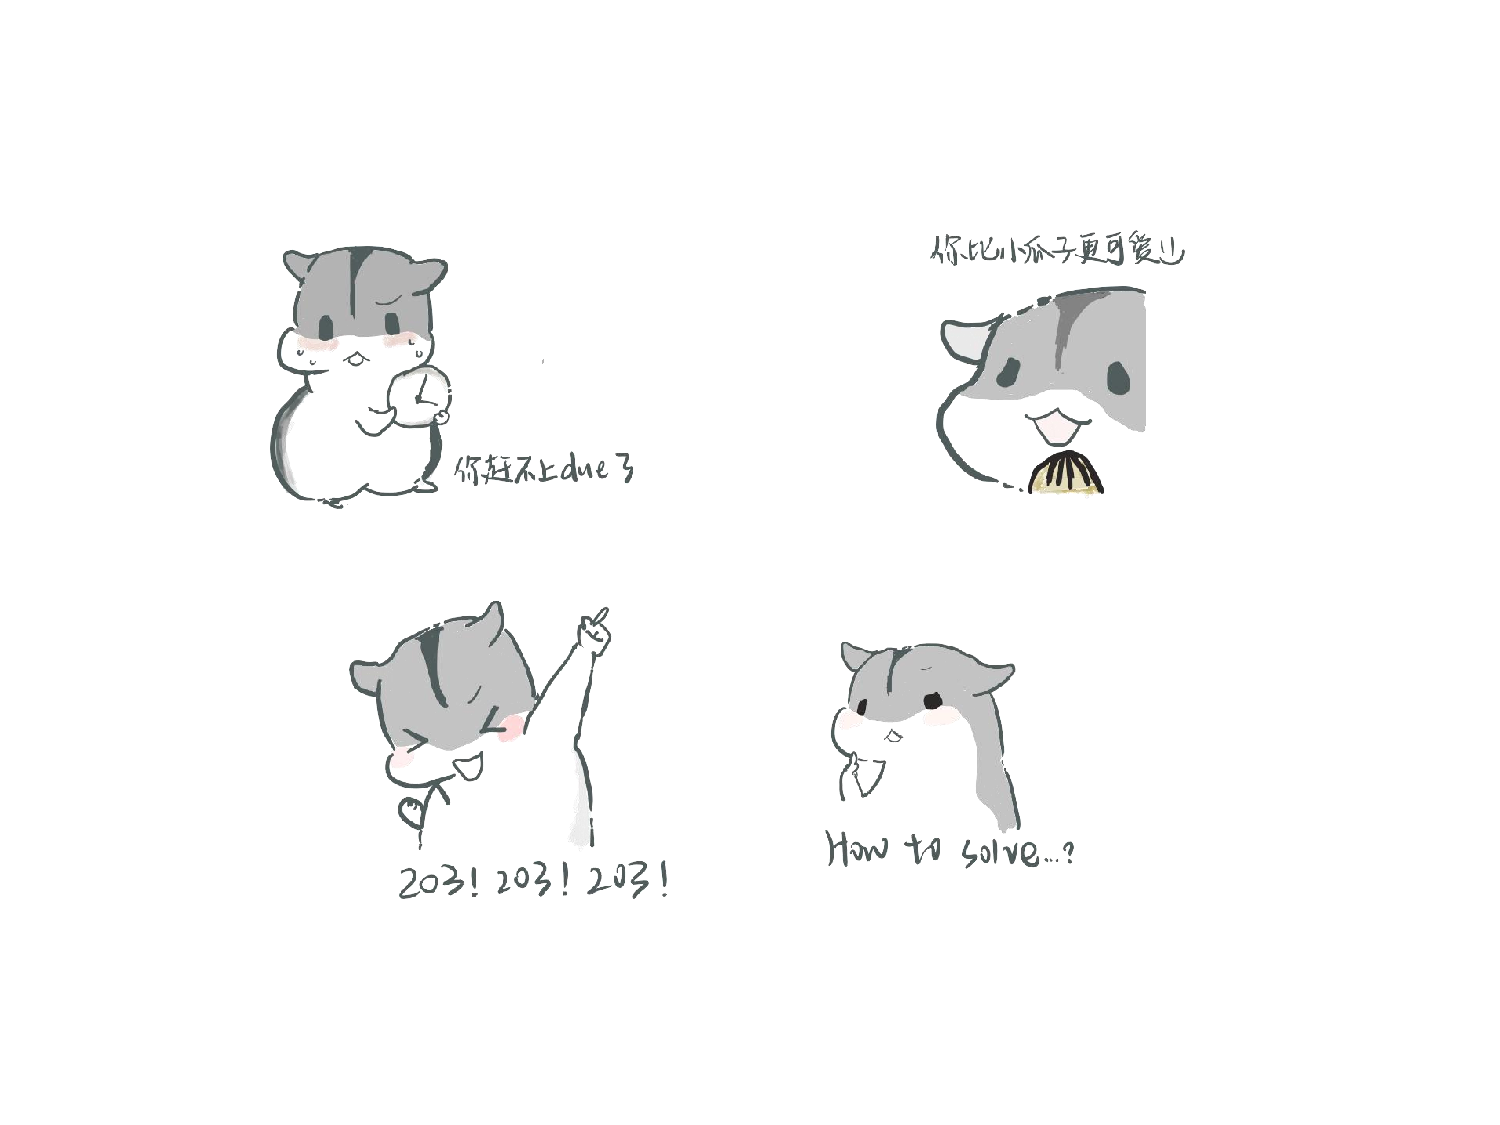
\includepdf[nup=1x1,scale=1.4]{new.pdf}
    \textcolor[rgb]{0.3,0.3,0.3}{\textbf{\huge{$\mathcal{Good~Luck~For~Your~Exam}$!}}}
\end{frame}
\usebackgroundtemplate{\tikz\node[opacity=0.25]{
    
\includegraphics[width=\paperwidth,
    height=\paperheight]{hamster.jpg}
    };}
\begin{frame}
    \frametitle{Reference}
    \begin{itemize}
        \item Content from Runze Cai's Slides.
        \item Content from Ve203-2021-fall Final RC by Xue Runze.
        \item Exericses from Ve203-2021-fall Final Exam.
        \item Exercises from Ve203-2021-summer Final Exam.
        \item Exercises from Ve203-2022-spring Homework 6.
        \item Exercises from Ve203-2020-fall Assignment 9.
        \item Cute paintings of Hamham from Wang Ruizhe.
    \end{itemize}
\end{frame}
\end{document}